% Appendix A

\chapter{Costruzione del dataset}
Nel ambito dei sistemi informatici geografici hanno una rilevanza importantissima i dataset di input. Su di essi infatti possono essere fatte le elaborazioni utili alla risoluzione e all'analisi di problematiche territoriali. Tali dati geografici purtroppo sono difficili da reperire e molto spesso non esistono. Questa difficoltà si traduce nel dover costruire il dataset. La costruzione può essere fatta in due modalità:
\begin{enumerate}
	\item Studio sul campo. Esso prevede di andare effettivamente sul territorio a campionare i dati. Tale metodo risulta molto costoso e lento.
	\item Costruzione sintetica del dataset. Questo modo di realizzazione usa dei dati preesistenti e attraverso elaborazioni restituisce un dataset conforme alle specifiche.
\end{enumerate}
Nel caso in esame non esistendo un dataset contenente i dati relativi all'esposizione al pericolo frane della regione Abruzzo, si è deciso di costruirne uno. Tale costruzione è stata fatta tenendo conto di diverse specifiche:
\begin{enumerate}
	\item Partizionamento completo. Tutto il territorio della regione Abruzzo deve essere partizionato in modo tale da non avere alcuna zona priva di un valore di esposizione al rischio. Ogni partizione verrà chiamata \textit{Zone}.
	\item Ogni \textit{Zone} deve avere associato un valore che esprime la pericolosità di quella particella rispetto al pericolo che essa frani. Tale valore è chiamato \textit{Szk}
	\item Ogni \textit{Zone} deve avere un area minima di 500 $m^2$
\end{enumerate}
Si è quindi proposta una prima soluzione. Essa verrà esplicitata seguendo una lista di passi.
\begin{enumerate}
	\item Creazione di una griglia di 155x155 elementi di lato 1 $km^2$ (fig.\ref{fig:griglia})
	\item Intersezione della griglia con la regione Abruzzo (fig.\ref{fig:abruzzoGriglia})
\end{enumerate}

\begin{figure}[h]
	\hspace{0.1\linewidth}
	\begin{minipage}[t]{0.30\linewidth}
		\centering
		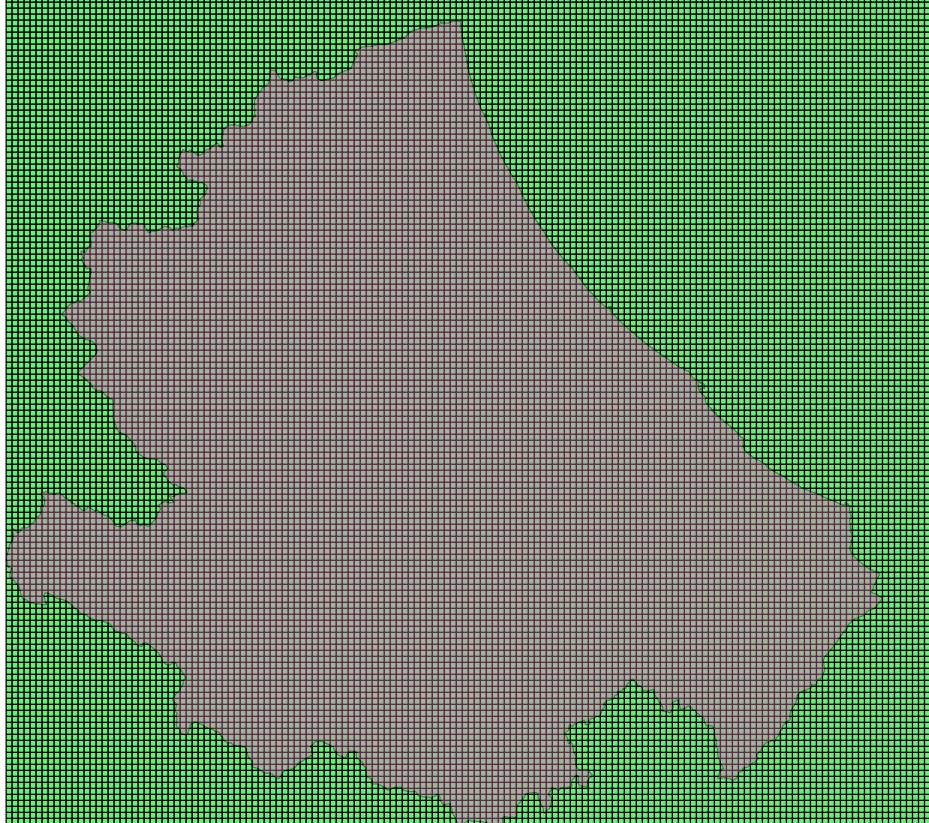
\includegraphics[width=\textwidth]{images/abruzzoQuadratini.PNG}
		\caption{}
		\label{fig:griglia}
	\end{minipage}
	\hspace{0.2\linewidth}
	\begin{minipage}[t]{0.30\linewidth}
		\centering
		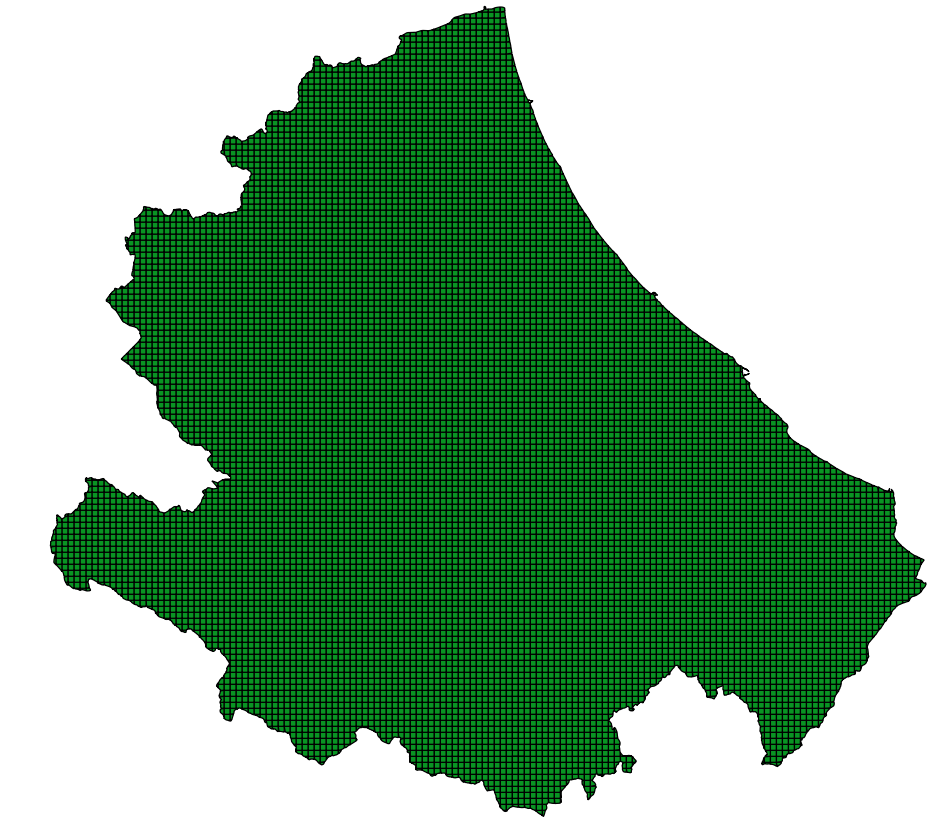
\includegraphics[width=\textwidth]{images/abruzzo.PNG}
		\caption{}
		\label{fig:abruzzoGriglia}
	\end{minipage}
\end{figure}
In primo momento si è proceduto ad assegnare un valore di \textit{Szk} casuale.
Tale valore però non avrebbe avuto una corrispondenza con la realtà e quindi qualsiasi risultato ottenuto con qualsiasi metodo sarebbe stato impossibile da validare. Si è quindi deciso che tale valore doveva essere deciso secondo una logica ben precisa.
Non avendo uno studio geologico completo di tutto il territorio abruzzese si è deciso di tenere in considerazione una sola variabile che contribuisce agli eventi franosi, ovvero la conformazione del suolo. Essa viene espressa attraverso delle curve di livello. Esse rappresentano tutti i punti a stessa quota sul territorio. La semplificazione ad una sola variabile permette di poter fare una validazione secondo una metrica ben precisa.
Le curve di livello  sono state ottenute a partire dai dati DEM del territorio abruzzese.
Tali dati sono stati reperiti sul portale USGS (United States Geological Survey). L'USGS è la maggiore agenzia per la cartografia civile degli Stati Uniti. I dati prelevati da tale portale sono quelli della missione NASA SRTM.
Lo Shuttle Radar Topography Mission (SRTM) è un'impresa internazionale che è riuscita ad ottenere un Modello digitale di elevazione su una scala quasi globale. 
\begin{figure}[h]
	\centering
	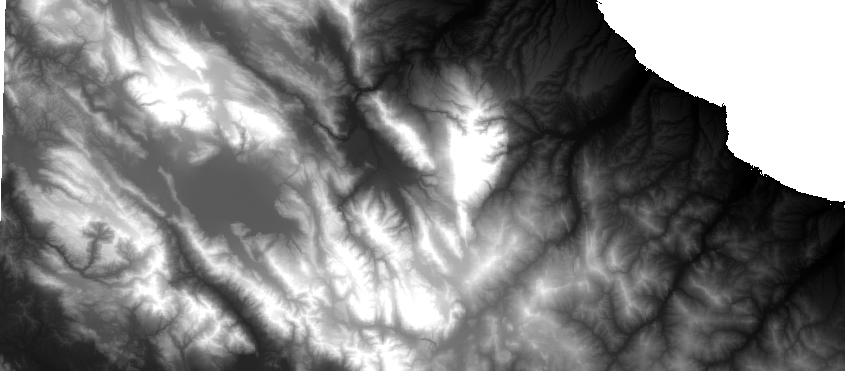
\includegraphics[width=1\textwidth]{images/STRM.PNG}
	\caption{In Figura si può osservare l'immagine raster del territorio abruzzese ottenuta dalla missione SRTM}
	\label{fig:diagrammaER}
\end{figure}

Lo SRTM consisteva in un sistema radar modificato che ha volato a bordo dello Space Shuttle Endeavour durante gli 11 giorni della missione STS-99 del febbraio 2000. Per acquisire i dati topografici dei dati di elevazione, il carico SRTM è stato equipaggiato con due antenne radar. Un'antenna era posizionata nello spazio di carico dello Shuttle, l'altra alla fine di un braccio di 60 metri che si estendeva dallo spazio di carico una volta che lo Shuttle era nello spazio. La tecnica impiegata è conosciuta come Interferometric Synthetic Aperture Radar. I modelli di elevazione ricavati dai dati dello SRTM vengono usati nei Geographic information system (GIS). Possono essere liberamente scaricati tramite internet ed il loro formato di file è supportato da parecchi programmi software. Sono stati prelevati i dati raster della regione Abruzzo e attraverso QGis (Software per la visualizzazione e l'elaborazione di dati geografici) sono state generate le curve di livello. Tali curve hanno una risoluzione di 25m. Infine sono state esportate come shape file.
\begin{figure}[h]
	\centering
	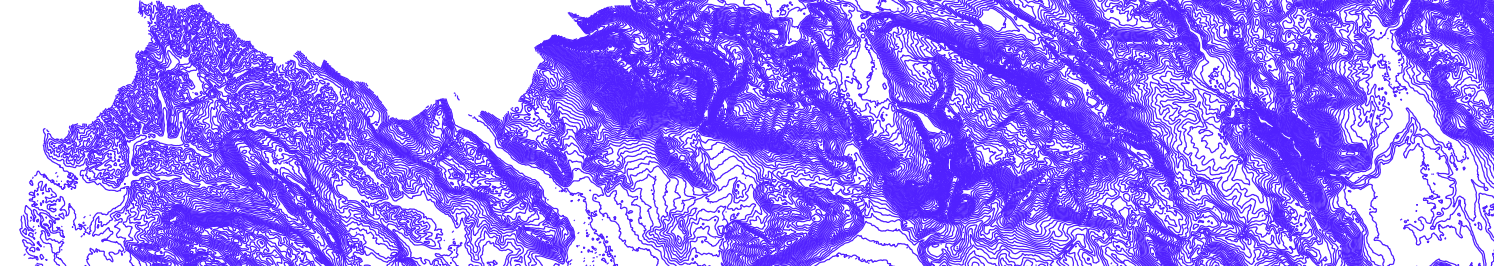
\includegraphics[width=1\textwidth]{images/dettaglioCurve.PNG}
	\caption{In figura si possono osservare le curve di livello di una porzione di territorio della regione Abruzzo}
	\label{fig:diagrammaER}
\end{figure}
Avendo introdotto le curve di livello (Isoipse) si sono decisi i valori di \textit{Szk} tenendo conto della morfologia effettiva del terreno. 
Per far ciò si e semplicemente contato il numero di curve di livello che intersecano ogni \textit{Zone}. Maggiore sono il numero di intersezioni maggiore sarà la ripidità del suolo quindi maggiore sarà il pericolo frana. Come detto in precedenza questa è una semplificazione estrema in quanto nella realtà ci sono moltissimi altri fattori che scatenano una frana. Si è quindi ottenuto un dataset che rimarcasse attraverso gli \textit{Szk} l'andamento del terreno.
\begin{figure}[h]
	\centering
	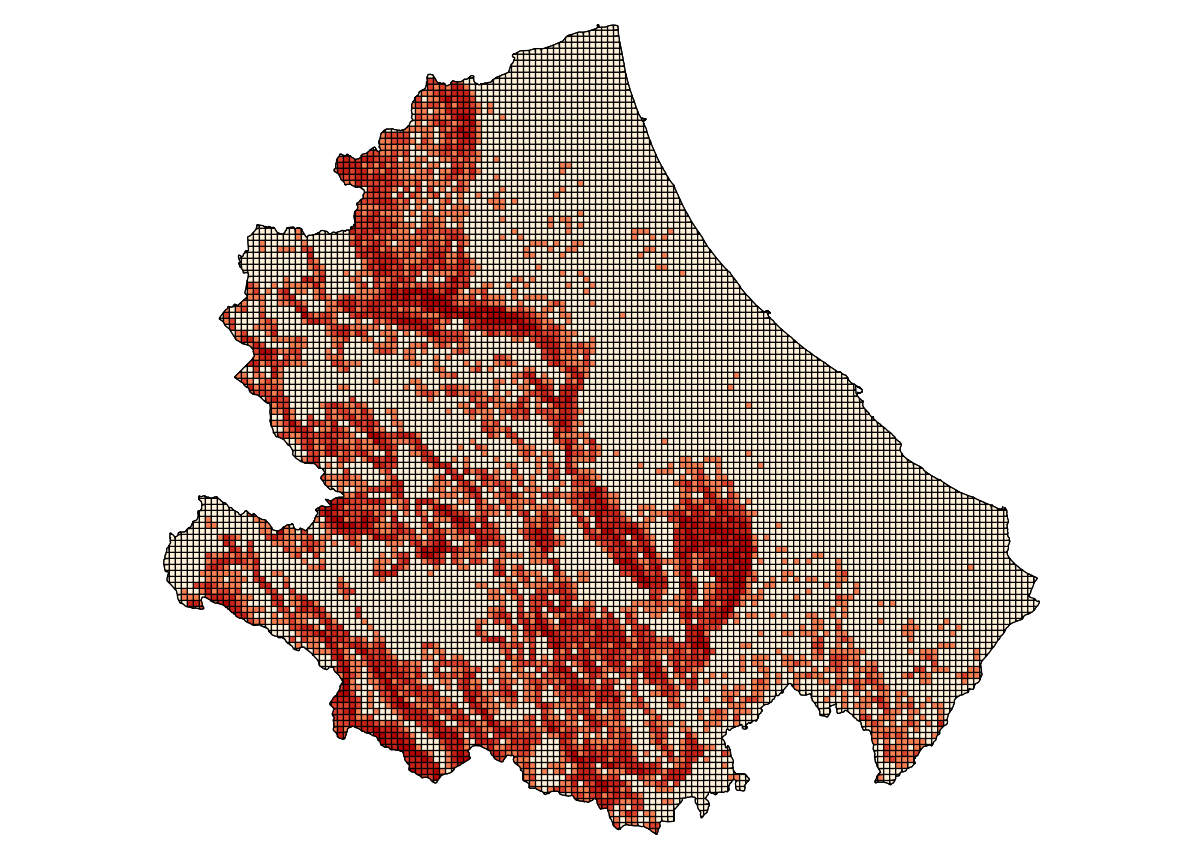
\includegraphics[width=1\textwidth]{images/abruzzoZKquadretto.png}
	\caption{In figura si può osservare il dataset ottenuto tenendo conto delle curve di livello}
	\label{fig:diagrammaER}
\end{figure}
Tale dataset ha due grandi limiti.
\begin{enumerate}
	\item Estrema regolarità delle \textit{Zone}
	\item Aree estremamente piccole lungo i bordi
\end{enumerate}
Per quanto riguarda il secondo limite si è risolto il problema aggregando le aree piccole a quelle vicine a loro. Essendo il primo limite troppo vincolante si è deciso di cambiare modello di generazione delle \textit{Zone}. Si è quindi provato ad usare il modello di Voronoi. In matematica, un diagramma di Voronoi (dal nome di Georgij Voronoi), anche detto tassellatura di Voronoi, decomposizione di Voronoi, o tassellatura di Dirichlet (dal nome di Lejeune Dirichlet) è un particolare tipo di decomposizione di uno spazio metrico determinata dalle distanze rispetto ad un determinato insieme discreto di elementi dello spazio (ad esempio, un insieme finito di punti). Il risultato ottenuto dall'unione della decomposizione di Voronoi con le curve di livello ha prodotto un risultato davvero soddisfacente. Il limite delle aree regolari si è superato in quanto tale tassellatura genera aree tutte differenti tra di loro. Mentre il limite delle aree molto piccole sui bordi non si presenta affatto.
Per aumentare la variazione \textit{Szk}  in pianura si è deciso di aggiungere un valore casuale.
\begin{figure}[h]
	\centering
	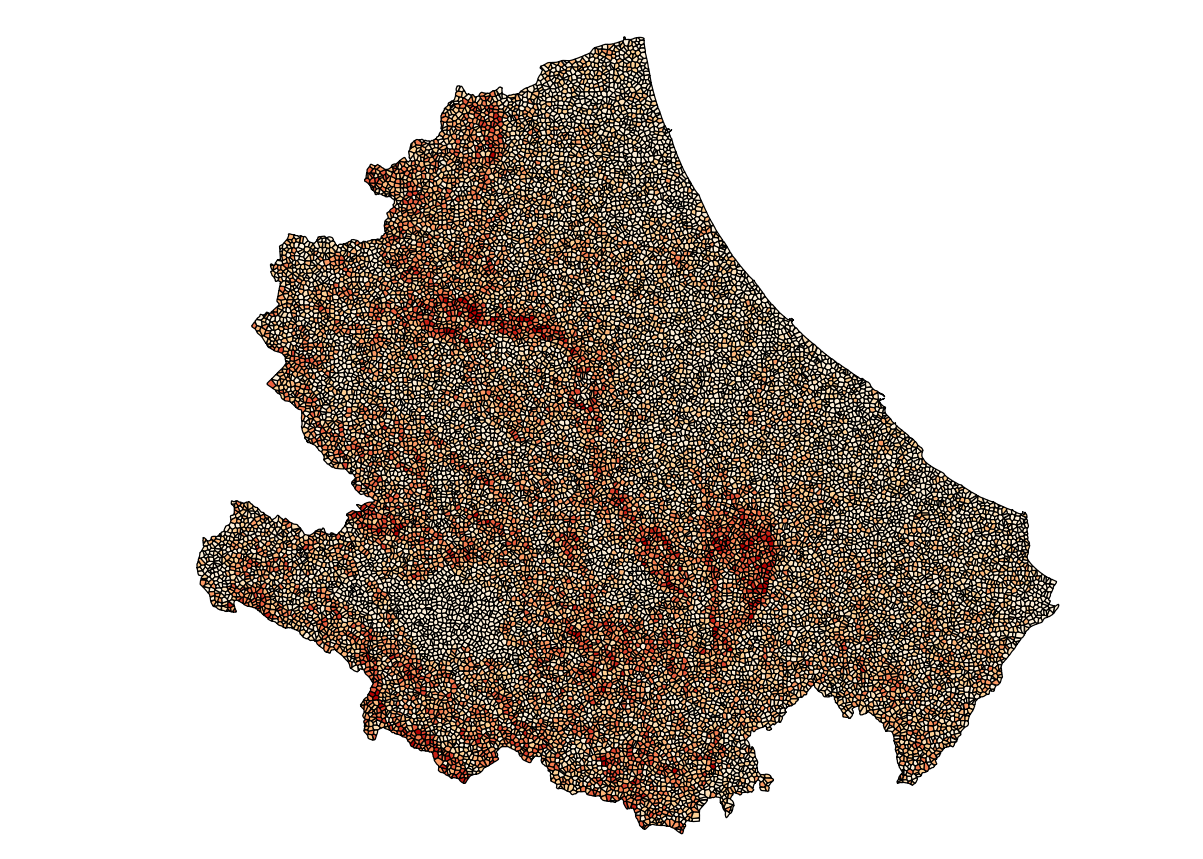
\includegraphics[width=1\textwidth]{images/voronoi.png}
	\caption{In figura si può osservare il dataset ottenuto tenendo conto delle curve di livello ed applicando la scomposizione di Voronoi}
	\label{fig:diagrammaER}
\end{figure}
In definitiva attraverso le curve di livello ricavate dai dati raster, la suddivisione in poligoni di Voronoi si è ottenuto un dataset sintetico che va a rispettare tutte le specifiche che ci eravamo imposti. Di seguito verranno proposte le UDF relative alla creazione del dataset.
\newpage
\hrule
\begin{lstlisting}
CREATE TABLE voronoi AS
SELECT (ST_DUMP(geom_voronoi)).geom AS geom_dump 
FROM (
SELECT ST_collectionextract(
ST_voronoipolygons(geom_point),3) AS geom_voronoi
FROM (
SELECT ST_GeneratePoints( geom , 22000) AS geom_point
FROM geo_area AS query3 
)AS query2
)AS query;

CREATE TABLE dataset AS
SELECT ST_Intersection(abruzzo.geom,voronoi.geom_dump) AS geom
FROM voronoi, geo_area AS abruzzo;



\end{lstlisting}
\hrule
\begin{lstlisting}
CREATE OR REPLACE FUNCTION zkcalcolus (idc INTEGER) RETURNS void
LANGUAGE plpgsql
AS $$
DECLARE
max INTEGER;
min INTEGER;
probabilita FLOAT;
diff FLOAT;
cursore RECORD;
posneg FLOAT;
variance FLOAT;
BEGIN
FOR cursore in SELECT id,geom FROM dataset WHERE idc = id LOOP
max := 0;
min := 0;
diff := 0;
probabilita := 0;
posneg := 0;
variance := 0;

CREATE TEMP TABLE intersezioneQuadratino
id SERIAL PRIMARY KEY , elevation float, geom geometry);

INSERT INTO intersezioneQuadratino(elevation, geom) 
SELECT isoipseabruzzo25.elevation,st_collectionextract(
st_intersection(dataset.geom,isoipseabruzzo25.geom),2) 
FROM isoipseabruzzo25,dataset
WHERE dataset.id = cursore.id;

CREATE TEMP TABLE intersezioneQuadratinoPulita
(id SERIAL PRIMARY KEY , elevation float, geom geometry);
INSERT INTO intersezioneQuadratinoPulita 
SELECT * 
FROM intersezioneQuadratino 
WHERE st_astext(geom) <> 'MULTILINESTRING EMPTY';

max :=( SELECT elevation 
FROM intersezioneQuadratinoPulita 
ORDER BY elevation DESC LIMIT 1);
min :=( SELECT elevation 
FROM intersezioneQuadratinoPulita 
ORDER BY elevation ASC LIMIT 1);

DROP TABLE intersezioneQuadratino;
DROP TABLE intersezioneQuadratinoPulita;

posneg :=(SELECT random());
IF posneg > 0.5 THEN
posneg = 1;
ELSE
posneg = -1;
END IF;
variance := (SELECT (random()*0.3));
variance := variance * posneg;
diff := max - min;
IF diff <> 0 THEN
IF diff > 800 THEN
probabilita := 1;
ELSE
probabilita := diff / 800 ;
probabilita := probabilita + variance;
IF probabilita > 1 THEN
probabilita := 1;
END IF;
IF probabilita < 0 THEN
probabilita := 0;
END IF;
END IF;
ELSE
probabilita := 0;
END IF ;
UPDATE dataset SET zk = probabilita WHERE id = cursore.id;
END LOOP;
END;
$$
\end{lstlisting}
\hrule